% Focused discussion: one purpose and one take-home claim per frame.
\begin{frame}[plain]
\vspace{.3cm}
{\LARGE\bfseries\color{ink}Which redox groups remain useful\\after grafting onto a polymer?}
\par\vspace{.6cm}
\begin{tikzpicture}[>=Latex,every node/.style={align=center,font=\large}]
\node[draw=teal,fill=soft,rounded corners,minimum height=1.35cm,text width=3.4cm] (a) {Design the\\redox motif};
\node[right=.5cm of a,draw=teal,fill=soft,rounded corners,minimum height=1.35cm,text width=3.4cm] (b) {Validate its\\computed properties};
\node[right=.5cm of b,draw=teal,fill=soft,rounded corners,minimum height=1.35cm,text width=3.4cm] (c) {Test attachment\\and neighbors};
\draw[->,very thick,teal] (a)--(b);\draw[->,very thick,teal] (b)--(c);
\end{tikzpicture}
\par\vspace{.6cm}\large Candidate expansion and validation: progress through 26 October 2026
\takeaway{The target is a useful grafted material, so molecular advantages must survive attachment and polymer context.}
\end{frame}

\begin{frame}{One exact design links the whole workflow}
\centering
\begin{tikzpicture}[>=Latex,every node/.style={align=center,font=\normalsize}]
\node[draw=teal,fill=soft,rounded corners,text width=3.1cm,minimum height=1.35cm] (a) {Define exact\newline molecular pairs};
\node[right=.6cm of a,draw=teal,fill=soft,rounded corners,text width=3.1cm,minimum height=1.35cm] (b) {Review precursor\newline and route};
\node[right=.6cm of b,draw=teal,fill=soft,rounded corners,text width=3.1cm,minimum height=1.35cm] (c) {Compute solution\newline redox states};
\node[below=.8cm of c,draw=teal,fill=soft,rounded corners,text width=3.1cm,minimum height=1.35cm] (d) {Test grafting\newline and neighbors};
\node[left=.6cm of d,draw=amber,fill=soft,rounded corners,text width=3.1cm,minimum height=1.35cm] (e) {Require a pass\newline on every axis};
\node[left=.6cm of e,draw=ink,fill=soft,rounded corners,text width=3.1cm,minimum height=1.35cm] (f) {Compare feasible\newline designs};
\draw[->,thick,teal] (a)--(b);\draw[->,thick,teal] (b)--(c);\draw[->,thick,teal] (c)--(d);
\draw[->,thick,teal] (d)--(e);\draw[->,thick,teal] (e)--(f);
\end{tikzpicture}
\takeaway{Exact identity and separate validation gates connect expansion to selection.}
\source{Current route: post-functionalization of a preformed benzyl-chloride polymer. Explicit method controls are kept separate.}
\end{frame}

\begin{frame}{The library is broad within three reduction-active cores}
\begin{columns}[c]
\begin{column}{.65\textwidth}\includegraphics[width=\linewidth]{\figdir library.pdf}\end{column}
\begin{column}{.31\textwidth}
{\Huge\color{teal}\bfseries 837}\par exact local designs\\[.7em]
{\Large\bfseries 1,593}\par generation recipes\\[.7em]
{\Large\bfseries 32}\par\small overlap designs with\par both computed potentials
\end{column}\end{columns}
\takeaway{Enumeration is systematic; equivalent recipes are retained while each exact product is counted once.}
\source{33 library graphs overlap the 75-candidate evaluated cohort; 32 have both computed potentials. This is not an 837-molecule quantum screen.}
\end{frame}

\begin{frame}{A matched comparison asks one chemical question}
\centering\includegraphics[width=.96\linewidth,height=4.25cm,keepaspectratio]{\figdir exact_variants.pdf}
\par\smallskip\large Same PMDI core, ethyl cap and local benzyl attachment; declared ring substitution changes.
\takeaway{Attach every variation to an exact baseline before interpreting its computed effect.}
\source{Exact graft-site molecular graphs from the checked candidate feed. The corresponding precursor graphs are retained separately.}
\end{frame}

\begin{frame}{Ring electronics shifts voltage more than these cap changes}
\centering\includegraphics[width=.99\linewidth,height=4.9cm,keepaspectratio]{\figdir matched_redox.pdf}
\takeaway{18 systematic contrasts quantify tuning across all three cores; they do not establish better material performance.}
\source{Matched solution potentials, each relative to its declared ethyl baseline. Circles: first step; squares: second step. All 26 cohort contrasts reproduce.}
\end{frame}

\begin{frame}{The next expansion should fill chemistry gaps}
\begin{columns}[T]
\begin{column}{.42\textwidth}
\textbf{Seven core families}\par\medskip
\colorbox{soft}{\parbox{.92\linewidth}{\large Viologen\quad PMDI\quad NDI\\[.6em]\textcolor{teal}{BQ\quad AQ\\[.6em]Phenothiazine\quad TEMPO}}}
\par\medskip\small Current systematic coverage emphasizes the first three.
\end{column}
\begin{column}{.54\textwidth}
\centering\textbf{Predeclared polymer-design comparison}\par\medskip
\begin{tabular}{lcc}\toprule & Flexible & Constrained\\\midrule
Baseline & $\square$ & $\square$\\[.6em]
Shielded & $\square$ & $\square$\\\bottomrule\end{tabular}
\par\medskip\small Four slots per core: 28.\\Six extra electronic contrasts: 34 total.
\end{column}\end{columns}
\takeaway{Test shielding and linker constraints as tradeoffs: reduced association can cost attachment access or capacity.}
\source{These are 34 planned slots, not 34 generated molecules. Exact graphs, routes and matched physical comparisons remain to be completed.}
\end{frame}

\begin{frame}{Validation has three distinct jobs}
\begin{columns}[T]
\begin{column}{.31\textwidth}\begin{block}{1. Numerical correctness}\large Is the stated quantity computed consistently?\par\medskip\small Geometry, spin, Hessian and balanced-cycle checks.\end{block}\end{column}
\begin{column}{.31\textwidth}\begin{block}{2. Experimental accuracy}\large Does it reproduce measured properties?\par\medskip\small 39 redox endpoints for exact free molecules in MeCN.\end{block}\end{column}
\begin{column}{.31\textwidth}\begin{block}{3. Model robustness}\large Does the conclusion survive reasonable choices?\par\medskip\small Basis, rotor treatment, reference, conformers and speciation.\end{block}\end{column}
\end{columns}
\takeaway{A calculation can be numerically correct while its chemical prediction remains uncertain.}
\source{The candidate reconstruction reports 628 arithmetic checks with zero discrepancies. These are bookkeeping checks, not experimental validation.}
\end{frame}

\begin{frame}{The measured redox benchmark is complete: 39 / 39}
\centering\includegraphics[width=.99\linewidth,height=4.75cm,keepaspectratio]{\figdir benchmark.pdf}
\par\smallskip\small\textbf{Unfitted MAE \BenchmarkMAE\ V; RMSE \BenchmarkRMSE\ V.}\quad30 molecules, 7 studies, MeCN.
\takeaway{This establishes a free-molecule error scale; exact grafts and polymer interactions need separate validation.}
\source{Retrospective panel; no fitted correction or outlier removal. Molecular-cluster 95\% MAE interval: 0.213--0.286 V. No NDI endpoint.}
\end{frame}

\begin{frame}{The benchmark error is structured, not just random}
\centering\includegraphics[width=.99\linewidth,height=4.8cm,keepaspectratio]{\figdir bias.pdf}
\takeaway{The first/second-step difference motivates reference and charge-state diagnostics; one Fc shift cannot fix step spacings.}
\source{Offset results are post hoc, molecule-held-out internal diagnostics. Primary potentials remain unfitted; a causal Fc correction is not established.}
\end{frame}

\begin{frame}{Basis and thermal controls quantify specific sensitivities}
\centering\includegraphics[width=.99\linewidth,height=4.75cm,keepaspectratio]{\figdir sensitivity.pdf}
\takeaway{These tested settings move potentials by tens of mV; missing conformers and experimental accuracy remain separate questions.}
\source{Neutral SVPD reoptimization/Hessians with existing anion and Fc fixed. Rotor spans use fixed structures, energies and spins. These are not prediction intervals.}
\end{frame}

\begin{frame}{A descriptor leader still has to pass every required axis}
\begin{columns}[c]
\begin{column}{.67\textwidth}\includegraphics[width=\linewidth,height=4.65cm,keepaspectratio]{\figdir descriptor_projection.pdf}\end{column}
\begin{column}{.29\textwidth}
{\Huge\bfseries\color{teal}8}\par descriptor-front models\\[.7em]
{\Huge\bfseries\color{amber}0}\par all-axis eligible\\[.7em]
\small Route, stability, accessibility and neighbor evidence remain incomplete.
\end{column}\end{columns}
\takeaway{A strong voltage or nominal capacity cannot compensate for an unacceptable attachment route or unwanted interaction.}
\source{Projection of a three-objective comparison over 56 molecular models. Nominal molecular capacity is not usable polymer capacity. Four application cutoffs remain unset.}
\end{frame}

\begin{frame}{A defined base shifts grafting thermodynamics across the panel}
\centering\includegraphics[width=.97\linewidth,height=4.55cm,keepaspectratio]{\figdir base_shift.pdf}
\par\smallskip\small For a fixed base/byproduct model: $\Delta G_{\rm base}=\Delta G_{\rm HCl\ reference}+C_{\rm base}$.
\takeaway{Keep base-required BQ candidates for testing; ranking is unchanged and absolute reaction signs remain conditional.}
\source{DBU: $C=-102.78$; DIPEA: $C=-70.98$ kJ/mol (separated ions). DBU capture differs from the MeCN pKa anchor; DIPEA remains conditional. No yield or barrier prediction.}
\end{frame}

\begin{frame}{One PMDI design now connects the molecular and polymer tests}
\begin{columns}[c]
\begin{column}{.42\textwidth}\includegraphics[width=\linewidth,height=3.4cm,keepaspectratio]{\figdir pmdi_model.pdf}\par\small Local model: 4-methylbenzyl/ethyl PMDI.\end{column}
\begin{column}{.55\textwidth}
\small\begin{tabular}{@{}ll@{}}\toprule
Redox in MeCN & $E_1=-1.076$, $E_2=-1.977$ V\\[.6em]
Precursor access & Exact source identified\\[.6em]
First graft, DBU & $-97.72$ / $-96.96$ kJ/mol\\[.6em]
Neighbor cycle & $-1.86$ kJ/mol\\\bottomrule
\end{tabular}\par\medskip\small Selectivity and redox retention after attachment remain unresolved.
\end{column}\end{columns}
\takeaway{The framework can trace one design through the calculations while retaining a conditional route decision.}
\source{First-graft values: sites 2 / 3 of a five-repeat model, separated ions. One minimum per graph; absolute signs retain base/speciation limits.}
\end{frame}

\begin{frame}{The polymer cycle measures a conditional neighbor effect}
\begin{columns}[c]
\begin{column}{.65\textwidth}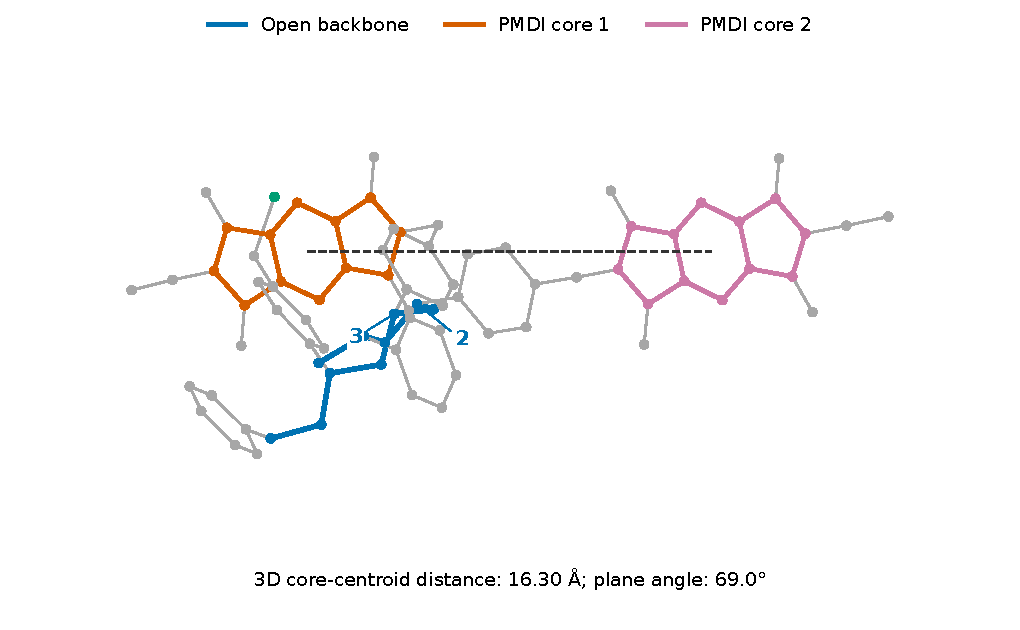
\includegraphics[width=\linewidth,height=4.6cm,keepaspectratio]{../results/figures/polymer_models/pmdi_neighbor_geometry.pdf}\end{column}
\begin{column}{.31\textwidth}
\Large $\Delta\Delta G =$\par\smallskip{\Huge\color{teal}$-1.86$}\par\large kJ/mol\par\medskip\normalsize Core separation: 16.30 \AA.\par\medskip\small Finite PMDI cycle in MeCN; one minimum for each graph.
\end{column}\end{columns}
\takeaway{This is whole-chain nonadditivity, not isolated motif binding or electronic coupling. Conformer convergence is still open.}
\source{$\Delta\Delta G=G_{11}+G_{00}-G_{10}-G_{01}$. Native Hessians and all four state sums independently reconstructed.}
\end{frame}

\begin{frame}{Since the reviewed draft, key gaps became checked results}
\begin{columns}[T]
\begin{column}{.46\textwidth}
\begin{block}{Measured benchmark}{\LARGE\bfseries39 / 39}\par\small Was 38 / 39. Bias and sensitivity analyses added.\end{block}
\begin{block}{Exact PMDI cycle}{\LARGE\bfseries$-1.86$ kJ/mol}\par\small Four-state native cycle now complete.\end{block}
\end{column}
\begin{column}{.46\textwidth}
\begin{block}{Spacing baseline}{\LARGE\bfseries6 / 6 selected $G$}\par\small Was 2 / 6. All 12 pose $G$ now available.\end{block}
\begin{block}{Portable raw replay}{\LARGE\bfseries14-state addendum}\par\small Native Hessians and cycles replay after relocation.\end{block}
\end{column}\end{columns}
\takeaway{Progress is in the completeness and defensibility of the evidence. Broader conformer convergence remains the main scientific gap.}
\source{Comparison uses the frozen 21 October manuscript snapshot, not an inferred reconstruction of live status on that date.}
\end{frame}

\begin{frame}{Next: convert molecular leaders into defensible material choices}
\begin{columns}[T]
\begin{column}{.31\textwidth}\begin{block}{Define useful performance}\large Set the operating window and minimum material capacity.\par\medskip\small Declare tolerable unwanted association and intersite coupling.\end{block}\end{column}
\begin{column}{.31\textwidth}\begin{block}{Broaden the chemistry}\large Fill the seven-core matched comparison panel.\par\medskip\small Review exact routes before expensive redox campaigns.\end{block}\end{column}
\begin{column}{.31\textwidth}\begin{block}{Bound polymer uncertainty}\large Finish conformer and backbone-configuration comparisons.\par\medskip\small Distinguish interaction energy, grafting nonadditivity and coupling.\end{block}\end{column}
\end{columns}
\takeaway{We have a linked, auditable workflow and concrete results; a synthesis shortlist requires all-axis evidence.}
\end{frame}
